
\phChapterWorksheet{Bonus Puzzle}{Catch Mobimon in the Expedition Zone!}

\begin{center}
  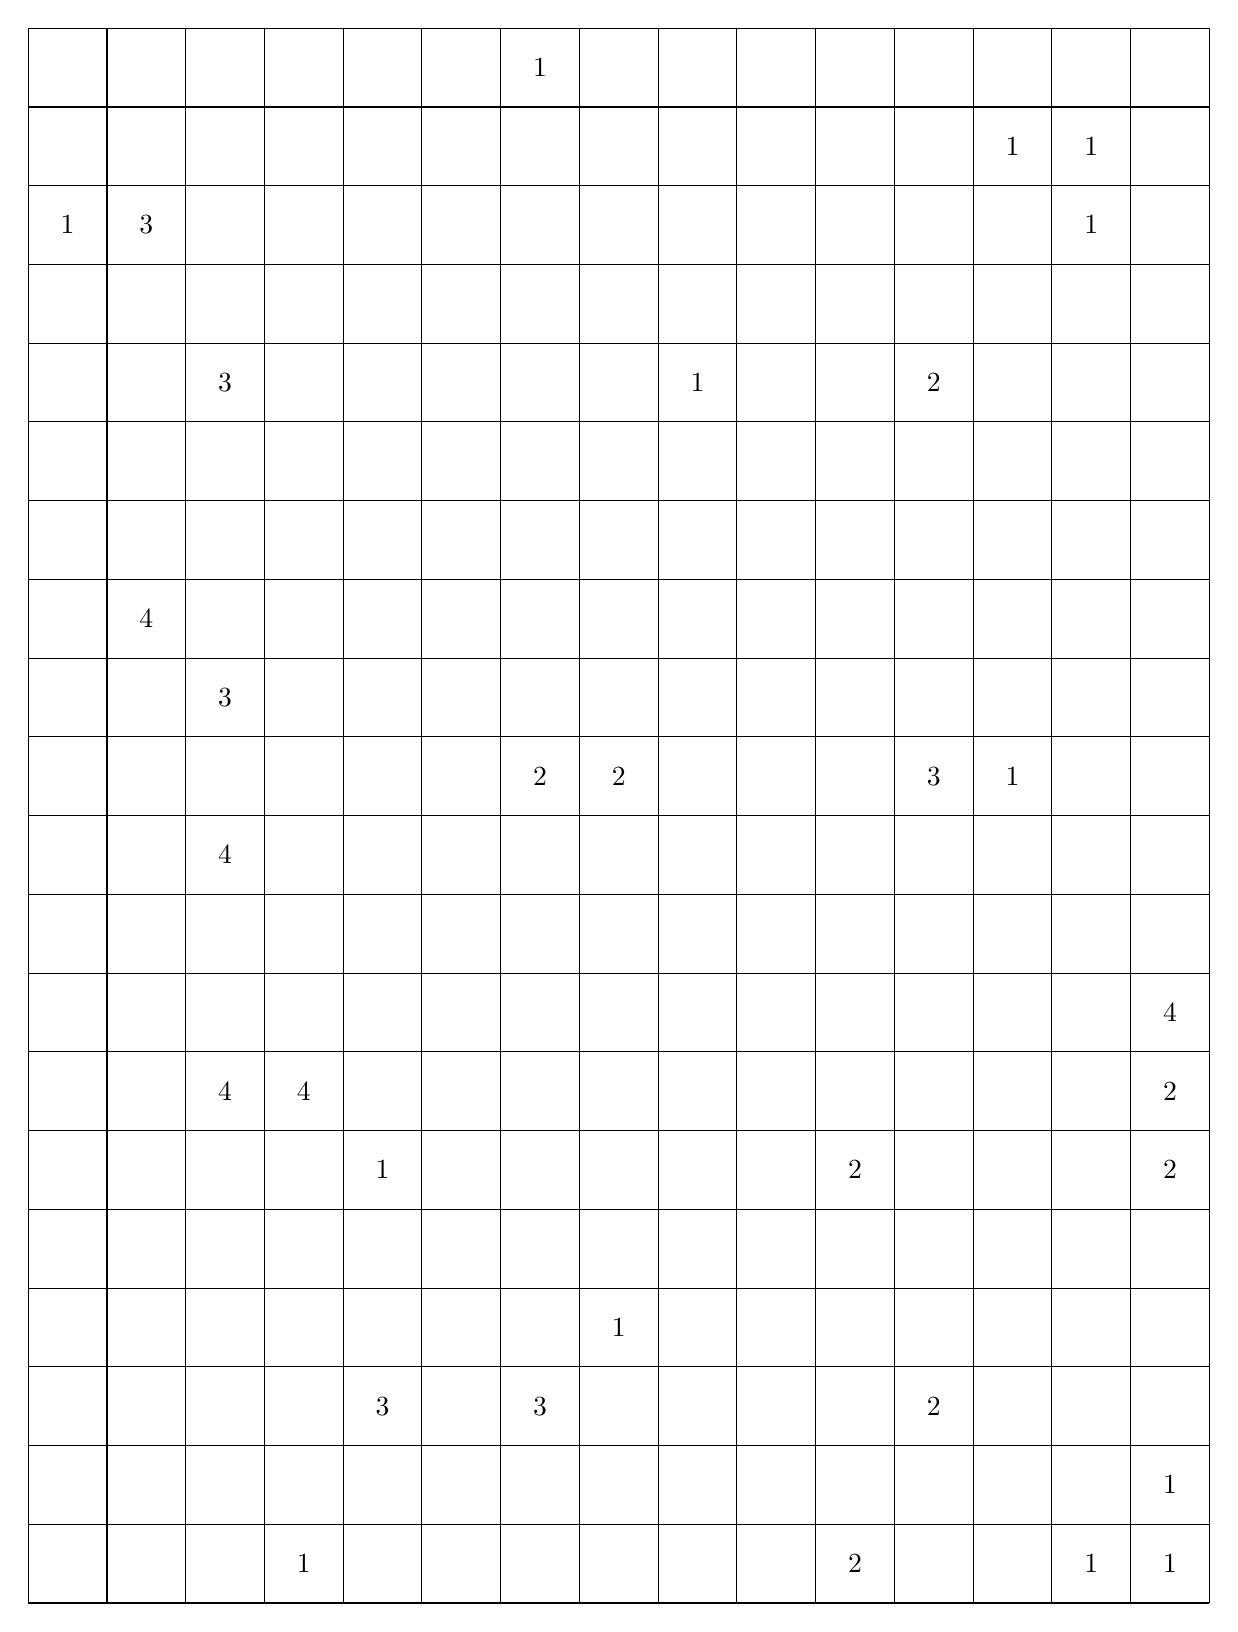
\begin{tikzpicture}
    %grid
    \draw[step=10mm] (0,0) grid (15,20);
    %nodes - randomly generated by gridgenerator.py
    %run the command:
    % > python gridgenerator.py
    %to generate a new set and copy/paste from gridgen.out (which is a text file
    %despite the unusual extension
    \node at (5mm, 175mm){1};
    \node at (15mm, 125mm){4};
    \node at (15mm, 175mm){3};
    \node at (25mm, 65mm){4};
    \node at (25mm, 95mm){4};
    \node at (25mm, 115mm){3};
    \node at (25mm, 155mm){3};
    \node at (35mm, 5mm){1};
    \node at (35mm, 65mm){4};
    \node at (45mm, 25mm){3};
    \node at (45mm, 55mm){1};
    \node at (65mm, 25mm){3};
    \node at (65mm, 105mm){2};
    \node at (65mm, 195mm){1};
    \node at (75mm, 35mm){1};
    \node at (75mm, 105mm){2};
    \node at (85mm, 155mm){1};
    \node at (105mm, 5mm){2};
    \node at (105mm, 55mm){2};
    \node at (115mm, 25mm){2};
    \node at (115mm, 105mm){3};
    \node at (115mm, 155mm){2};
    \node at (125mm, 105mm){1};
    \node at (125mm, 185mm){1};
    \node at (135mm, 5mm){1};
    \node at (135mm, 175mm){1};
    \node at (135mm, 185mm){1};
    \node at (145mm, 5mm){1};
    \node at (145mm, 15mm){1};
    \node at (145mm, 55mm){2};
    \node at (145mm, 65mm){2};
    \node at (145mm, 75mm){4};
  \end{tikzpicture}
\end{center}

% Include below for aucTeX integration
%%% Local Variables:
%%% mode: latex
%%% TeX-master: "../mapp-challenge-18-game-book"
%%% End:
